\begin{quote}\small\textbf{观课提示}\quad 逐次匹配值、斜率和更高导数，观察近似在离开中心后怎样变化。

\href{https://www.youtube.com/watch?v=3d6DsjIBzJ4}{原课程视频}\quad\href{https://vitael04213.github.io/3blue1brown-notes/lessons/taylor-series.html}{本节网页与媒体}\quad\href{https://vitael04213.github.io/3blue1brown-notes/lab.html\#taylor}{参数实验}
\end{quote}
\begin{figure}[htbp]\centering
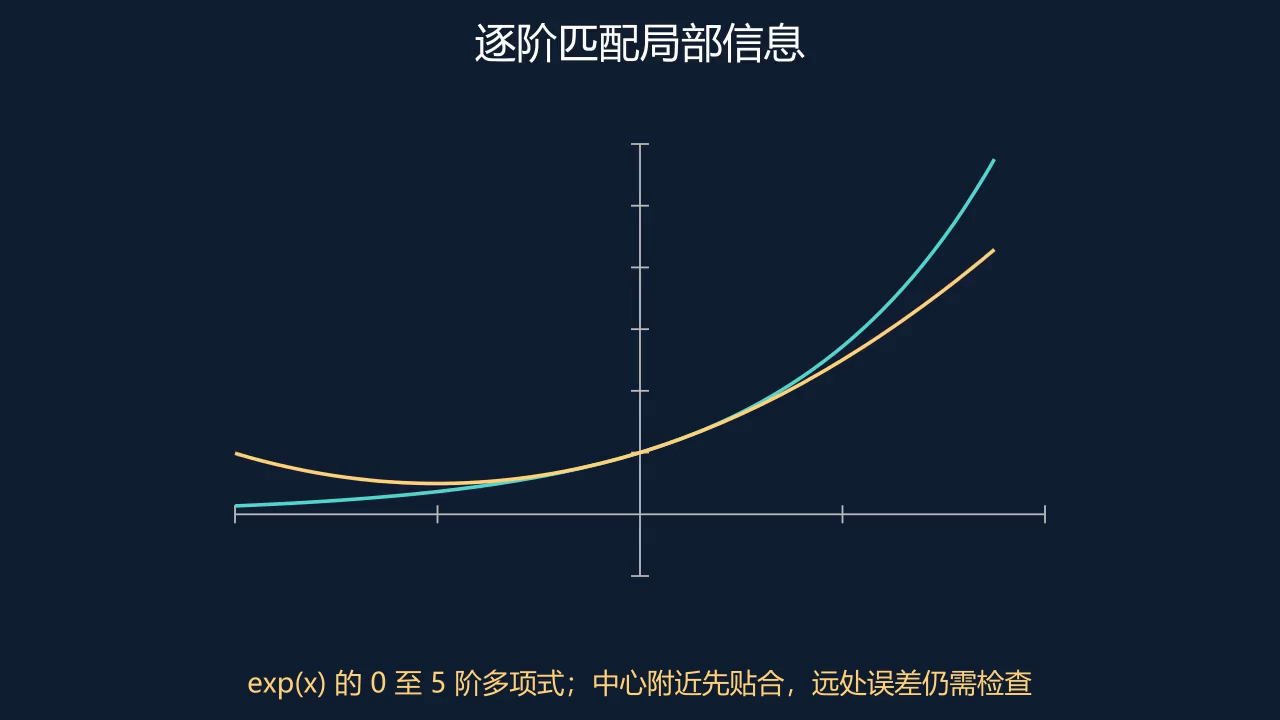
\includegraphics[width=0.98\linewidth]{figures/Taylor.png}
\caption{指数函数（蓝）与逐阶泰勒多项式（黄）；精度需要结合离中心距离判断。本项目原创 Manim 动画关键帧；完整动画与操作入口见本节网页。}
\end{figure}
